\documentclass[a4paper,11pt]{report}

\usepackage{amsmath}
\usepackage{fullpage}
\usepackage{tikz}

\usetikzlibrary{graphs,graphs.standard}

\makeatletter
\pgfmathdeclarefunction{alpha}{1}{%
  \pgfmathint@{#1}%
  \edef\pgfmathresult{\pgffor@alpha{\pgfmathresult}}%
}

\usepackage{bussproofs}
\usepackage{mathpartir}
\usepackage{prooftrees}
\usepackage{color}

\usepackage{tikz}
\usetikzlibrary{automata,positioning}

\author{Sylvain Julmy}
\date{\today}

\setlength{\parindent}{0pt}

\begin{document}

\begin{center}
  \Large{
    Mathematical Methods for Computer Science 2\
    Spring 2018
  }
  \noindent\makebox[\linewidth]{\rule{\linewidth}{0.4pt}}

  Series 6
  \vspace*{1.4cm}

  Sylvain Julmy
  
  \noindent\makebox[\linewidth]{\rule{\linewidth}{0.4pt}}
\end{center}

\section*{\texttt{1}}

\subsection*{a)}

We consider that $0$ is divisible by $2$ and by $3$.

\begin{center}
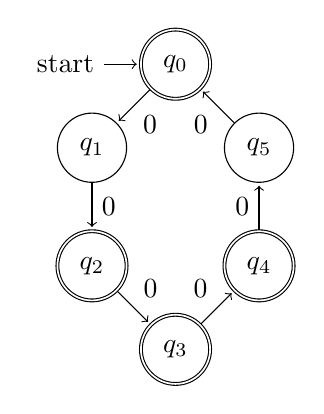
\begin{tikzpicture}[shorten >=1pt,node distance=1.5cm,on grid,auto]
\node[state,initial,accepting] (q0) {$q_0$};
\node[state] (q1) [below left = of q0] {$q_1$};
\node[state,accepting] (q2) [below = of q1] {$q_2$};
\node[state,accepting] (q3) [below right = of q2] {$q_3$};
\node[state] (q5) [below right = of q0] {$q_5$};
\node[state,accepting] (q4) [below = of q5] {$q_4$};
\path[->]
(q0) edge [] node [] {$0$} (q1)
(q1) edge [] node [] {$0$} (q2)
(q2) edge [] node [] {$0$} (q3)
(q3) edge [] node [] {$0$} (q4)
(q4) edge [] node [] {$0$} (q5)
(q5) edge [] node [] {$0$} (q0)
;
\end{tikzpicture}
\end{center}

\subsection*{b)}

\begin{center}
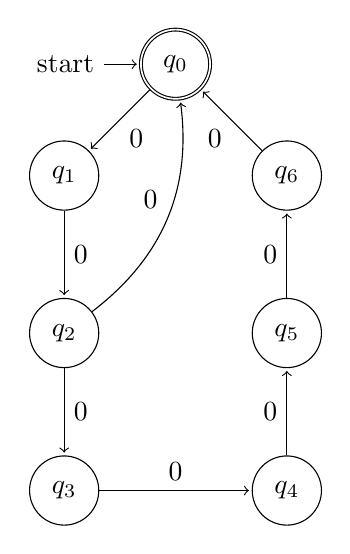
\begin{tikzpicture}[shorten >=1pt,node distance=2cm,on grid,auto]
  \node[state,initial,accepting] (q0) {$q_0$};
  \node[state] (q1) [below left = of q0] {$q_1$};
  \node[state] (q2) [below = of q1] {$q_2$};
  \node[state] (q3) [below = of q2] {$q_3$};
  \node[state] (q6) [below right = of q0] {$q_6$};
  \node[state] (q5) [below = of q6] {$q_5$};
  \node[state] (q4) [below = of q5] {$q_4$};
  \path[->]
  (q0) edge [] node [] {$0$} (q1)
  (q1) edge [] node [] {$0$} (q2)
  (q2) edge [] node [] {$0$} (q3)
       edge [bend right] node [] {$0$} (q0)
  (q3) edge [] node [] {$0$} (q4)
  (q4) edge [] node [] {$0$} (q5)
  (q5) edge [] node [] {$0$} (q6)
  (q6) edge [] node [] {$0$} (q0)
  ;
\end{tikzpicture}
\end{center}

\section*{\texttt{2}}

\subsection*{a)}

\begin{center}
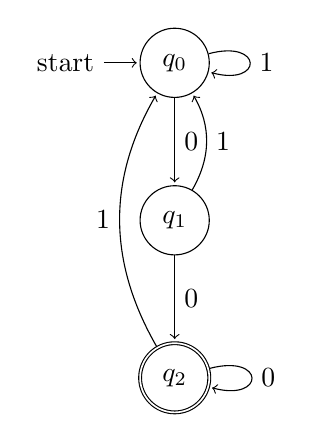
\begin{tikzpicture}[shorten >=1pt,node distance=2cm,on grid,auto]
  \node[state,initial] (q0) {$q_0$};
  \node[state] (q1) [below = of q0] {$q_1$};
  \node[state,accepting] (q2) [below = of q1] {$q_2$};
  \path[->]
  (q0)
  edge [loop right] node [] {$1$} ()
  edge [] node [] {${0}$} (q1)
  (q1)
  edge [bend right] node [right] {$1$} (q0)
  edge [] node [] {${0}$} (q2)
  (q2)
  edge [loop right] node [] {$0$} ()
  edge [bend left] node [] {$1$} (q0)
  ;
\end{tikzpicture}
\end{center}

\subsection*{b)}

\begin{center}
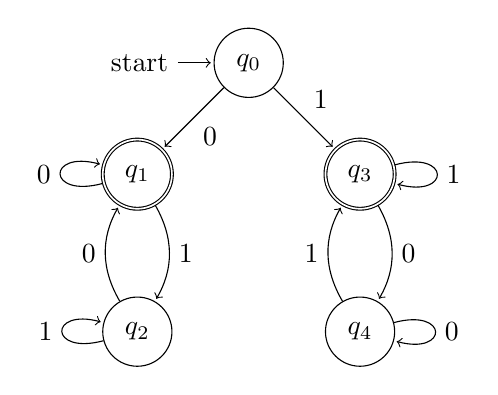
\begin{tikzpicture}[shorten >=1pt,node distance=2cm,on grid,auto]
  \node[state,initial] (q0) {$q_0$};
  \node[state,accepting] (q1) [below left = of q0] {$q_1$};
  \node[state] (q2) [below  = of q1] {$q_2$};
  \node[state,accepting] (q3) [below right = of q0] {$q_3$};
  \node[state] (q4) [below  = of q3] {$q_4$};
  \path[->]
  (q0)
  edge [] node [] {$0$} (q1)
  edge [] node [] {$1$} (q3)
  (q1)
  edge [loop left] node [] {$0$} ()
  edge [bend left] node [] {$1$} (q2)
  (q2)
  edge [bend left] node [] {$0$} (q1)
  edge [loop left] node [] {$1$} ()
  (q3)
  edge [loop right] node [] {$1$} ()
  edge [bend left] node [] {$0$} (q4)
  (q4)
  edge [bend left] node [] {$1$} (q3)
  edge [loop right] node [] {$0$} ()
  ;
\end{tikzpicture}
\end{center}

\subsection*{c)}

Each state represent a number from $0$ to $4$ (the rest of the division by $5$)
and then we encode the number from $0$ to $9$ in order to recover the correct
result after the division by $5$. If $n \equiv 0 \mod 5$ then it binary string
reach state $q_0$.

\begin{center}
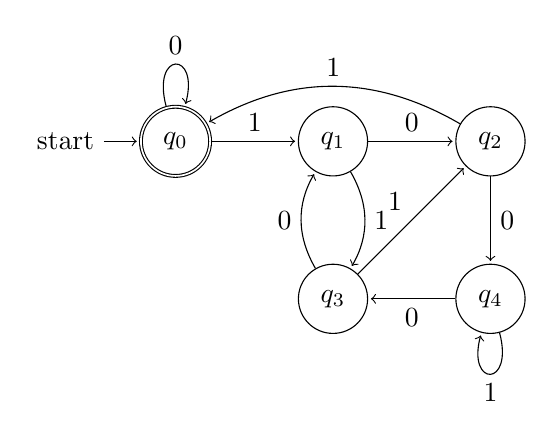
\begin{tikzpicture}[shorten >=1pt,node distance=2cm,on grid,auto]
  \node[state,initial,accepting] (q0) {$q_0$};
  \node[state] (q1) [right = of q0] {$q_1$};
  \node[state] (q2) [right = of q1] {$q_2$};
  \node[state] (q3) [below = of q1] {$q_3$};
  \node[state] (q4) [below = of q2] {$q_4$};
  \path[->]
  (q0)
  edge [loop above] node [] {$0$} ()
  edge [] node [] {$1$} (q1)
  (q1)
  edge [] node [] {$0$} (q2)
  edge [bend left] node [] {$1$} (q3)
  (q2)
  edge [] node [] {$0$} (q4)
  edge [bend right] node [above] {$1$} (q0)
  (q3)
  edge [bend left] node [] {$0$} (q1)
  edge [] node [] {$1$} (q2)
  (q4)
  edge [] node [] {$0$} (q3)
  edge [loop below] node [] {$1$} ()
  ;
\end{tikzpicture}
\end{center}

\section*{\texttt{3}}

Note : we label with $[0-9]$ the transitions when we encounter a digit and by
$[a-z]$ the ones when we encounter a letter. We also denote by $\Sigma^*$ any
possible symbol from the alphabet.

\subsection*{a)}
\begin{center}
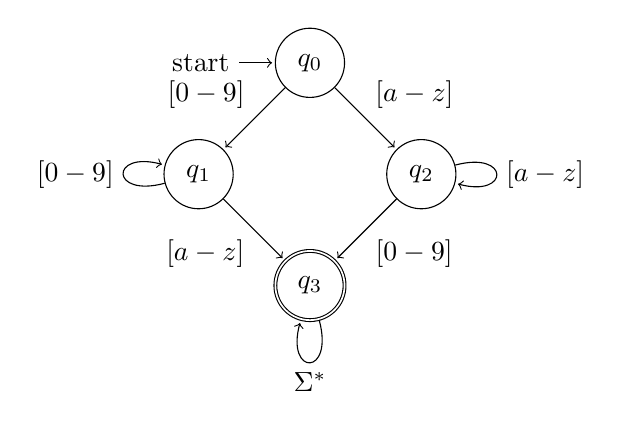
\begin{tikzpicture}[shorten >=1pt,node distance=2cm,on grid,auto]
  \node[state,initial] (q0) {$q_0$};
  \node[state] (q1) [below left = of q0] {$q_1$};
  \node[state] (q2) [below right = of q0] {$q_2$};
  \node[state,accepting] (q3) [below left = of q2] {$q_3$};
  \path[->]
  (q0)
  edge [] node [above left] {$[0-9]$} (q1)
  edge [] node [] {$[a-z]$} (q2)
  (q1)
  edge [loop left] node [] {$[0-9]$} ()
  edge [] node [below left] {$[a-z]$} (q3)
  (q2)
  edge [loop right] node [] {$[a-z]$} ()
  edge [] node [] {$[0-9]$} (q3)
  (q3)
  edge [loop below] node [] {$\Sigma^*$} ()
  ;
\end{tikzpicture}
\end{center}

\subsection*{b)}
\begin{center}
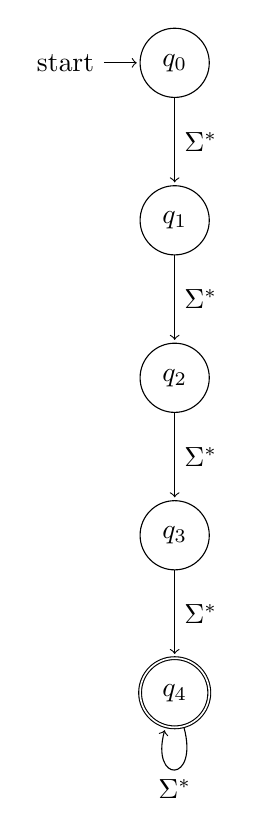
\begin{tikzpicture}[shorten >=1pt,node distance=2cm,on grid,auto]
  \node[state,initial] (q0) {$q_0$};
  \node[state] (q1) [below = of q0] {$q_1$};
  \node[state] (q2) [below = of q1] {$q_2$};
  \node[state] (q3) [below = of q2] {$q_3$};
  \node[state,accepting] (q4) [below = of q3] {$q_4$};
  \path[->]
  (q0) edge [] node [] {$\Sigma^*$} (q1)
  (q1) edge [] node [] {$\Sigma^*$} (q2)
  (q2) edge [] node [] {$\Sigma^*$} (q3)
  (q3) edge [] node [] {$\Sigma^*$} (q4)
  (q4)
  edge [loop below] node [] {$\Sigma^*$} ()
  ;
\end{tikzpicture}
\end{center}

\subsection*{c)}
\begin{center}
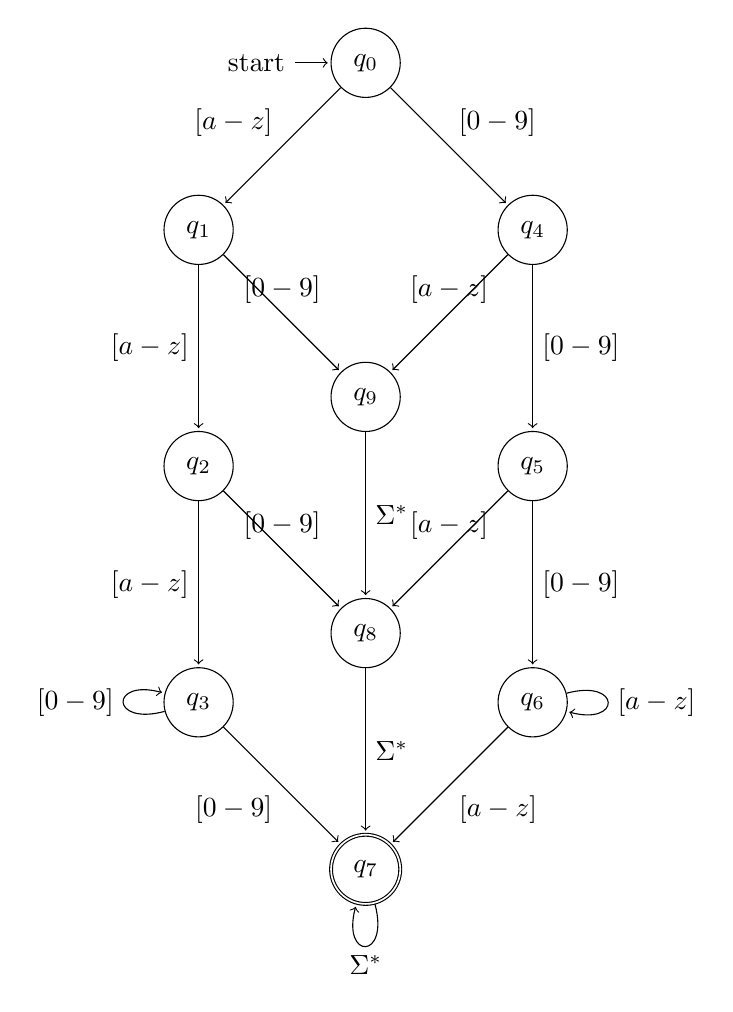
\begin{tikzpicture}[shorten >=1pt,node distance=3cm,on grid,auto]
  \node[state,initial] (q0) {$q_0$};
  \node[state] (q1) [below left = of q0] {$q_1$};
  \node[state] (q2) [below = of q1] {$q_2$};
  \node[state] (q3) [below = of q2] {$q_3$};
  \node[state] (q4) [below right = of q0] {$q_4$};
  \node[state] (q5) [below = of q4] {$q_5$};
  \node[state] (q6) [below = of q5] {$q_6$};
  \node[state,accepting] (q7) [below left = of q6] {$q_7$};
  \node[state] (q8) [above = of q7] {$q_8$};
  \node[state] (q9) [above = of q8] {$q_9$};
  \path[->]
  (q0)
  edge [] node [above left] {$[a-z]$} (q1)
  edge [] node [above right] {$[0-9]$} (q4)
  (q1)
  edge [] node [left] {$[a-z]$} (q2)
  edge [] node [above ] {$[0-9]$} (q9)
  (q2)
  edge [] node [left] {$[a-z]$} (q3)
  edge [] node [above ] {$[0-9]$} (q8)
  (q3)
  edge [] node [below left] {$[0-9]$} (q7)
  edge [loop left] node [] {$[0-9]$} ()
  (q4) 
  edge [] node [right] {$[0-9]$} (q5)
  edge [] node [above ] {$[a-z]$} (q9)
  (q5)
  edge [] node [right] {$[0-9]$} (q6)
  edge [] node [above ] {$[a-z]$} (q8)
  (q6)
  edge [] node [] {$[a-z]$} (q7)
  edge [loop right] node [] {$[a-z]$} ()
  (q7)
  edge [loop below] node [] {$\Sigma^*$} ()
  (q9) edge []  node [] {$\Sigma^*$} (q8)
  (q8) edge []  node [] {$\Sigma^*$} (q7)
  ;
\end{tikzpicture}
\end{center}

\section*{\texttt{4}}

\[
  \begin{array}{c|cc}
    & 0 & 1 \\ \hline
    \{p\} & \{p,q\} & \{p\} \\
    \{p,q\} & \{p,q,r\} & \{p,r\} \\
    \{p,q,r\} & \{p,q,r,s\} & \{p,r\}\\
    \{p,r\} & \{p,q,s\} & \{p\} \\
    \{p,q,s\} & \{p,q,s\} & \{p,r\}\\
    \{p,q,r,s\} & \{p,q,r,s\} & \{p,r\}\\
  \end{array}
\]


\begin{center}
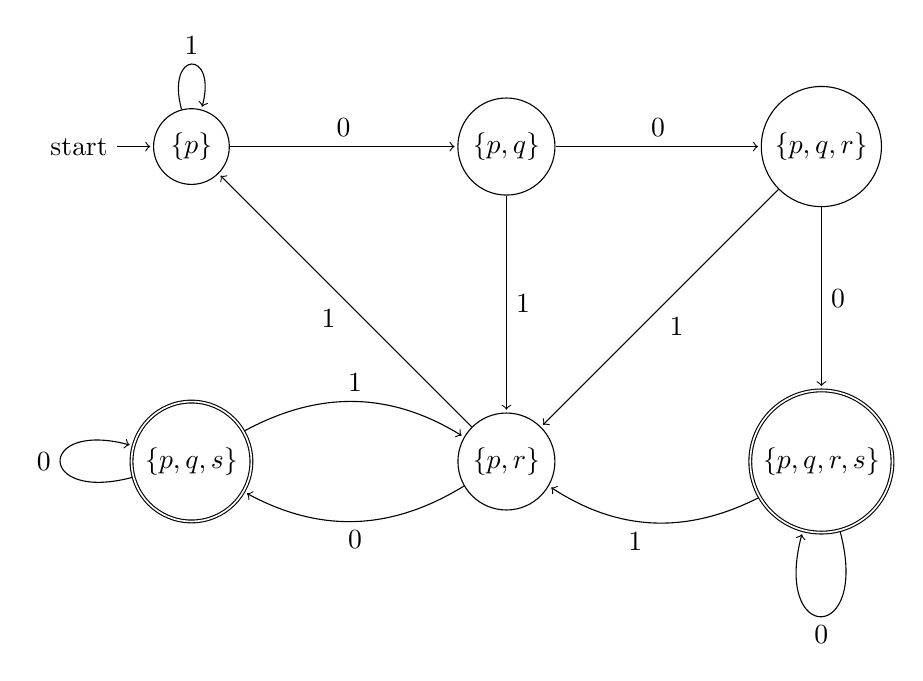
\begin{tikzpicture}[shorten >=1pt,node distance=4cm,on grid,auto]
  \node[state,initial] (q0) {$\{p\}$};
  \node[state] (q1) [right = of q0] {$\{p,q\}$};
  \node[state] (q2) [right = of q1] {$\{p,q,r\}$};
  \node[state] (q3) [below = of q1] {$\{p,r\}$};
  \node[state,accepting] (q4) [below = of q0] {$\{p,q,s\}$};
  \node[state,accepting] (q5) [below = of q2] {$\{p,q,r,s\}$};
  \path[->]
  (q0)
  edge [] node [] {$0$} (q1)
  edge [loop above] node [] {$1$} ()
  (q1)
  edge [] node [] {$0$} (q2)
  edge [] node [] {$1$} (q3)
  (q2)
  edge [] node [] {$0$} (q5)
  edge [] node [] {$1$} (q3)
  (q3)
  edge [bend left] node [] {$0$} (q4)
  edge [] node [] {$1$} (q0)
  (q4)
  edge [loop left] node [] {$0$} ()
  edge [bend left] node [] {$1$} (q3)
  (q5)
  edge [loop below] node [] {$0$} ()
  edge [bend left] node [] {$1$} (q3)
  ;
\end{tikzpicture}
\end{center}

And we can merge the two accepting state :

\begin{center}
\begin{tikzpicture}[shorten >=1pt,node distance=4cm,on grid,auto]
  \node[state,initial] (q0) {$\{p\}$};
  \node[state] (q1) [right = of q0] {$\{p,q\}$};
  \node[state] (q2) [right = of q1] {$\{p,q,r\}$};
  \node[state] (q3) [below = of q1] {$\{p,r\}$};
  \node[state,accepting] (q5) [below = of q2] {$\{p,q,r,s\} \cup \{p,q,s\}$};
  \path[->]
  (q0)
  edge [] node [] {$0$} (q1)
  edge [loop above] node [] {$1$} ()
  (q1)
  edge [] node [] {$0$} (q2)
  edge [] node [] {$1$} (q3)
  (q2)
  edge [] node [] {$0$} (q5)
  edge [] node [] {$1$} (q3)
  (q3)
  edge [bend left] node [] {$0$} (q5)
  edge [] node [] {$1$} (q0)
  (q5)
  edge [loop below] node [] {$0$} ()
  edge [bend left] node [] {$1$} (q3)
  ;
\end{tikzpicture}
\end{center}


\section*{\texttt{5}}

The NFA :

\begin{center}
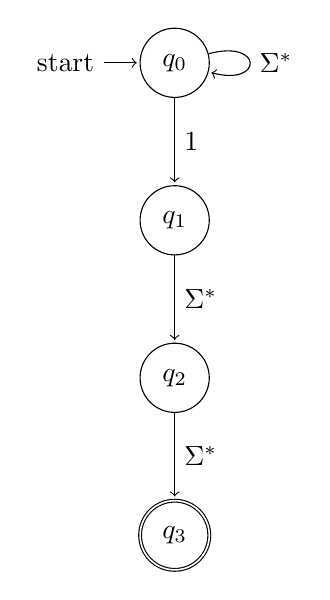
\begin{tikzpicture}[shorten >=1pt,node distance=2cm,on grid,auto]
  \node[state,initial] (q0) {$q_0$};
  \node[state] (q1) [below = of q0] {$q_1$};
  \node[state] (q2) [below = of q1] {$q_2$};
  \node[state,accepting] (q3) [below = of q2] {$q_3$};
  \path[->]
  (q0)
  edge [loop right] node [] {$\Sigma^*$} ()
  edge [] node [] {$1$} (q1)
  (q1) edge [] node [] {$\Sigma^*$} (q2)
  (q2) edge [] node [] {$\Sigma^*$} (q3)
  ;
\end{tikzpicture}
\end{center}

Transition tables :

\[
  \begin{array}{c|cc}
    & 0 & 1 \\ \hline
    q_0 & \{q_0\} & \{q_0,q_1\} \\
    q_1 & \{q_2\} & \{q_2\}\\
    q_2 & \{q_3\} & \{q_3\}\\
    q_3 & \emptyset & \emptyset\\
  \end{array}
\]

\[
  \begin{array}{c|cc}
    & 0 & 1 \\ \hline
    \{q_0\} & \{q_0\} & \{q_0,q_1\} \\
    \{q_0,q_1\} & \{q_0,q_2\} & \{q_0,q_1,q_2\} \\
    \{q_0,q_2\} & \{q_0,q_3\} & \{q_0,q_1,q_3\} \\
    \{q_0,q_1,q_2\} & \{q_0,q_2,q_3\} & \{q_0,q_1,q_2,q_3\} \\
    \{q_0,q_3\} & \{q_0\} & \{q_0,q_1\} \\
    \{q_0,q_1,q_3\} & \{q_0,q_2\} & \{q_0,q_1,q_2\} \\
    \{q_0,q_2,q_3\} & \{q_0,q_3\} & \{q_0,q_1,q_3\} \\
    \{q_0,q_1,q_2,q_3\} & \{q_0,q_2,q_3\} & \{q_0,q_1,q_2,q_3\} \\
  \end{array}
\]

\begin{center}
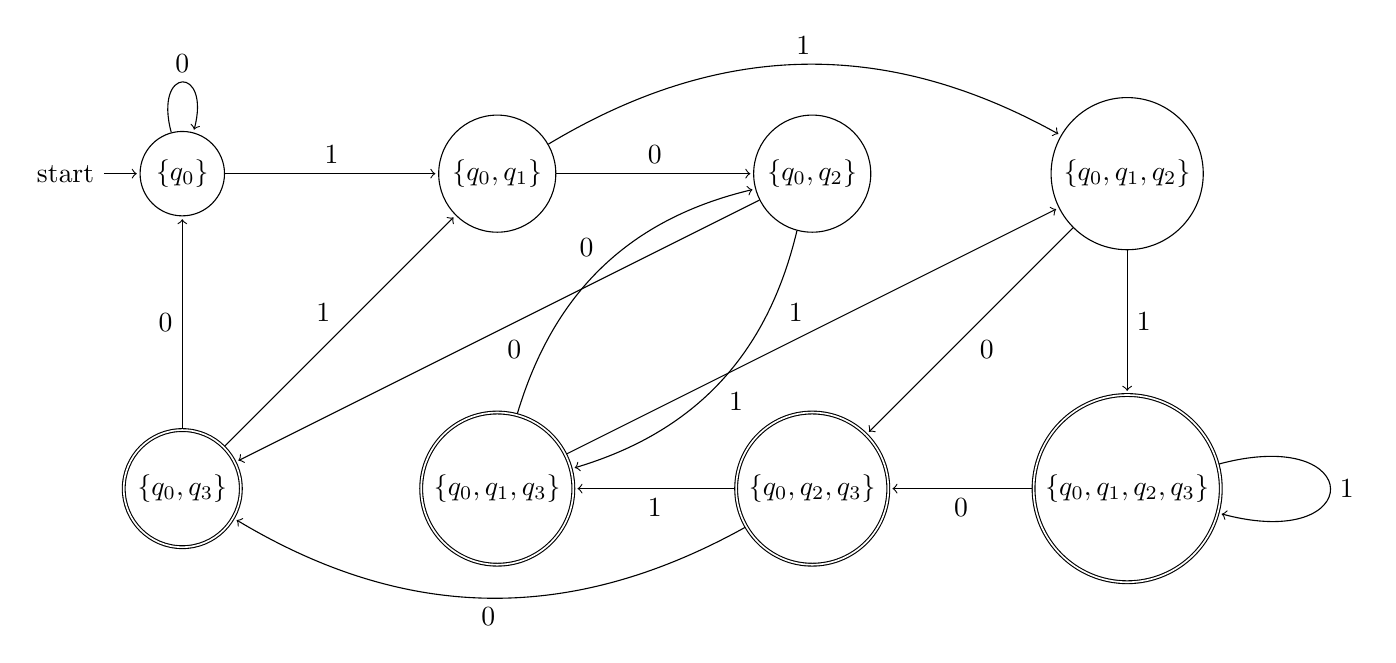
\begin{tikzpicture}[shorten >=1pt,node distance=4cm,on grid,auto]
  \node[state,initial] (q0) {$\{q_0\}$};
  \node[state] (q1) [right = of q0] {$\{q_0,q_1\}$};
  \node[state] (q2) [right = of q1] {$\{q_0,q_2\}$};
  \node[state] (q3) [right = of q2] {$\{q_0,q_1,q_2\}$};
  \node[state,accepting] (q4) [below = of q0] {$\{q_0,q_3\}$};
  \node[state,accepting] (q5) [below = of q1] {$\{q_0,q_1,q_3\}$};
  \node[state,accepting] (q6) [below = of q2] {$\{q_0,q_2,q_3\}$};
  \node[state,accepting] (q7) [below = of q3] {$\{q_0,q_1,q_2,q_3\}$};
  \path[->]
  (q0)
  edge [loop above] node [] {$0$} ()
  edge [] node [] {$1$} (q1)
  (q1)
  edge [] node [] {$0$} (q2)
  edge [bend left] node [] {$1$} (q3)
  (q2)
  edge [] node [] {$0$} (q4)
  edge [bend left] node [] {$1$} (q5)
  (q3)
  edge [] node [] {$0$} (q6)
  edge [] node [] {$1$} (q7)
  (q4)
  edge [] node [] {$0$} (q0)
  edge [] node [] {$1$} (q1)
  (q5)
  edge [bend left] node [] {$0$} (q2)
  edge [] node [] {$1$} (q3)
  (q6)
  edge [bend left] node [] {$0$} (q4)
  edge [] node [] {$1$} (q5)
  (q7)
  edge [] node [] {$0$} (q6)
  edge [loop right] node [] {$1$} ()
  ;
\end{tikzpicture}
\end{center}

We can't proceed further reduction on the state because we can't merge accepting
and non-accepting states.






\end{document}